\section{Objetivo}
Realizar programa que realice una secuencia que prenda y apague dos LED detectando el accionar del un botón por flanco. El programa principal debe mantener encendido el primer LED y al detectarse la pulsación del botón realizar una rutina de parpadeo en el segundo de los LED mientras el otro se apague. Al final la rutina de parpadeo, el primer LED se volverá a encender.

\section{Descripción del proyecto}
Se realizar\'a un programa en lenguaje \textit{Assembly} para la familia de microcontroladores \textit{AVR}.
Se utilizara la plataforma \textit{Arduino} y el \textit{Shield I/O} para utilizar las conexiones de dos LED y un botón pulsador, en función de esto se eligieron los puertos de entrada y salida.


\begin{figure}[ht]
\begin{minipage}{.45\textwidth}
  \centering
  % include first image
  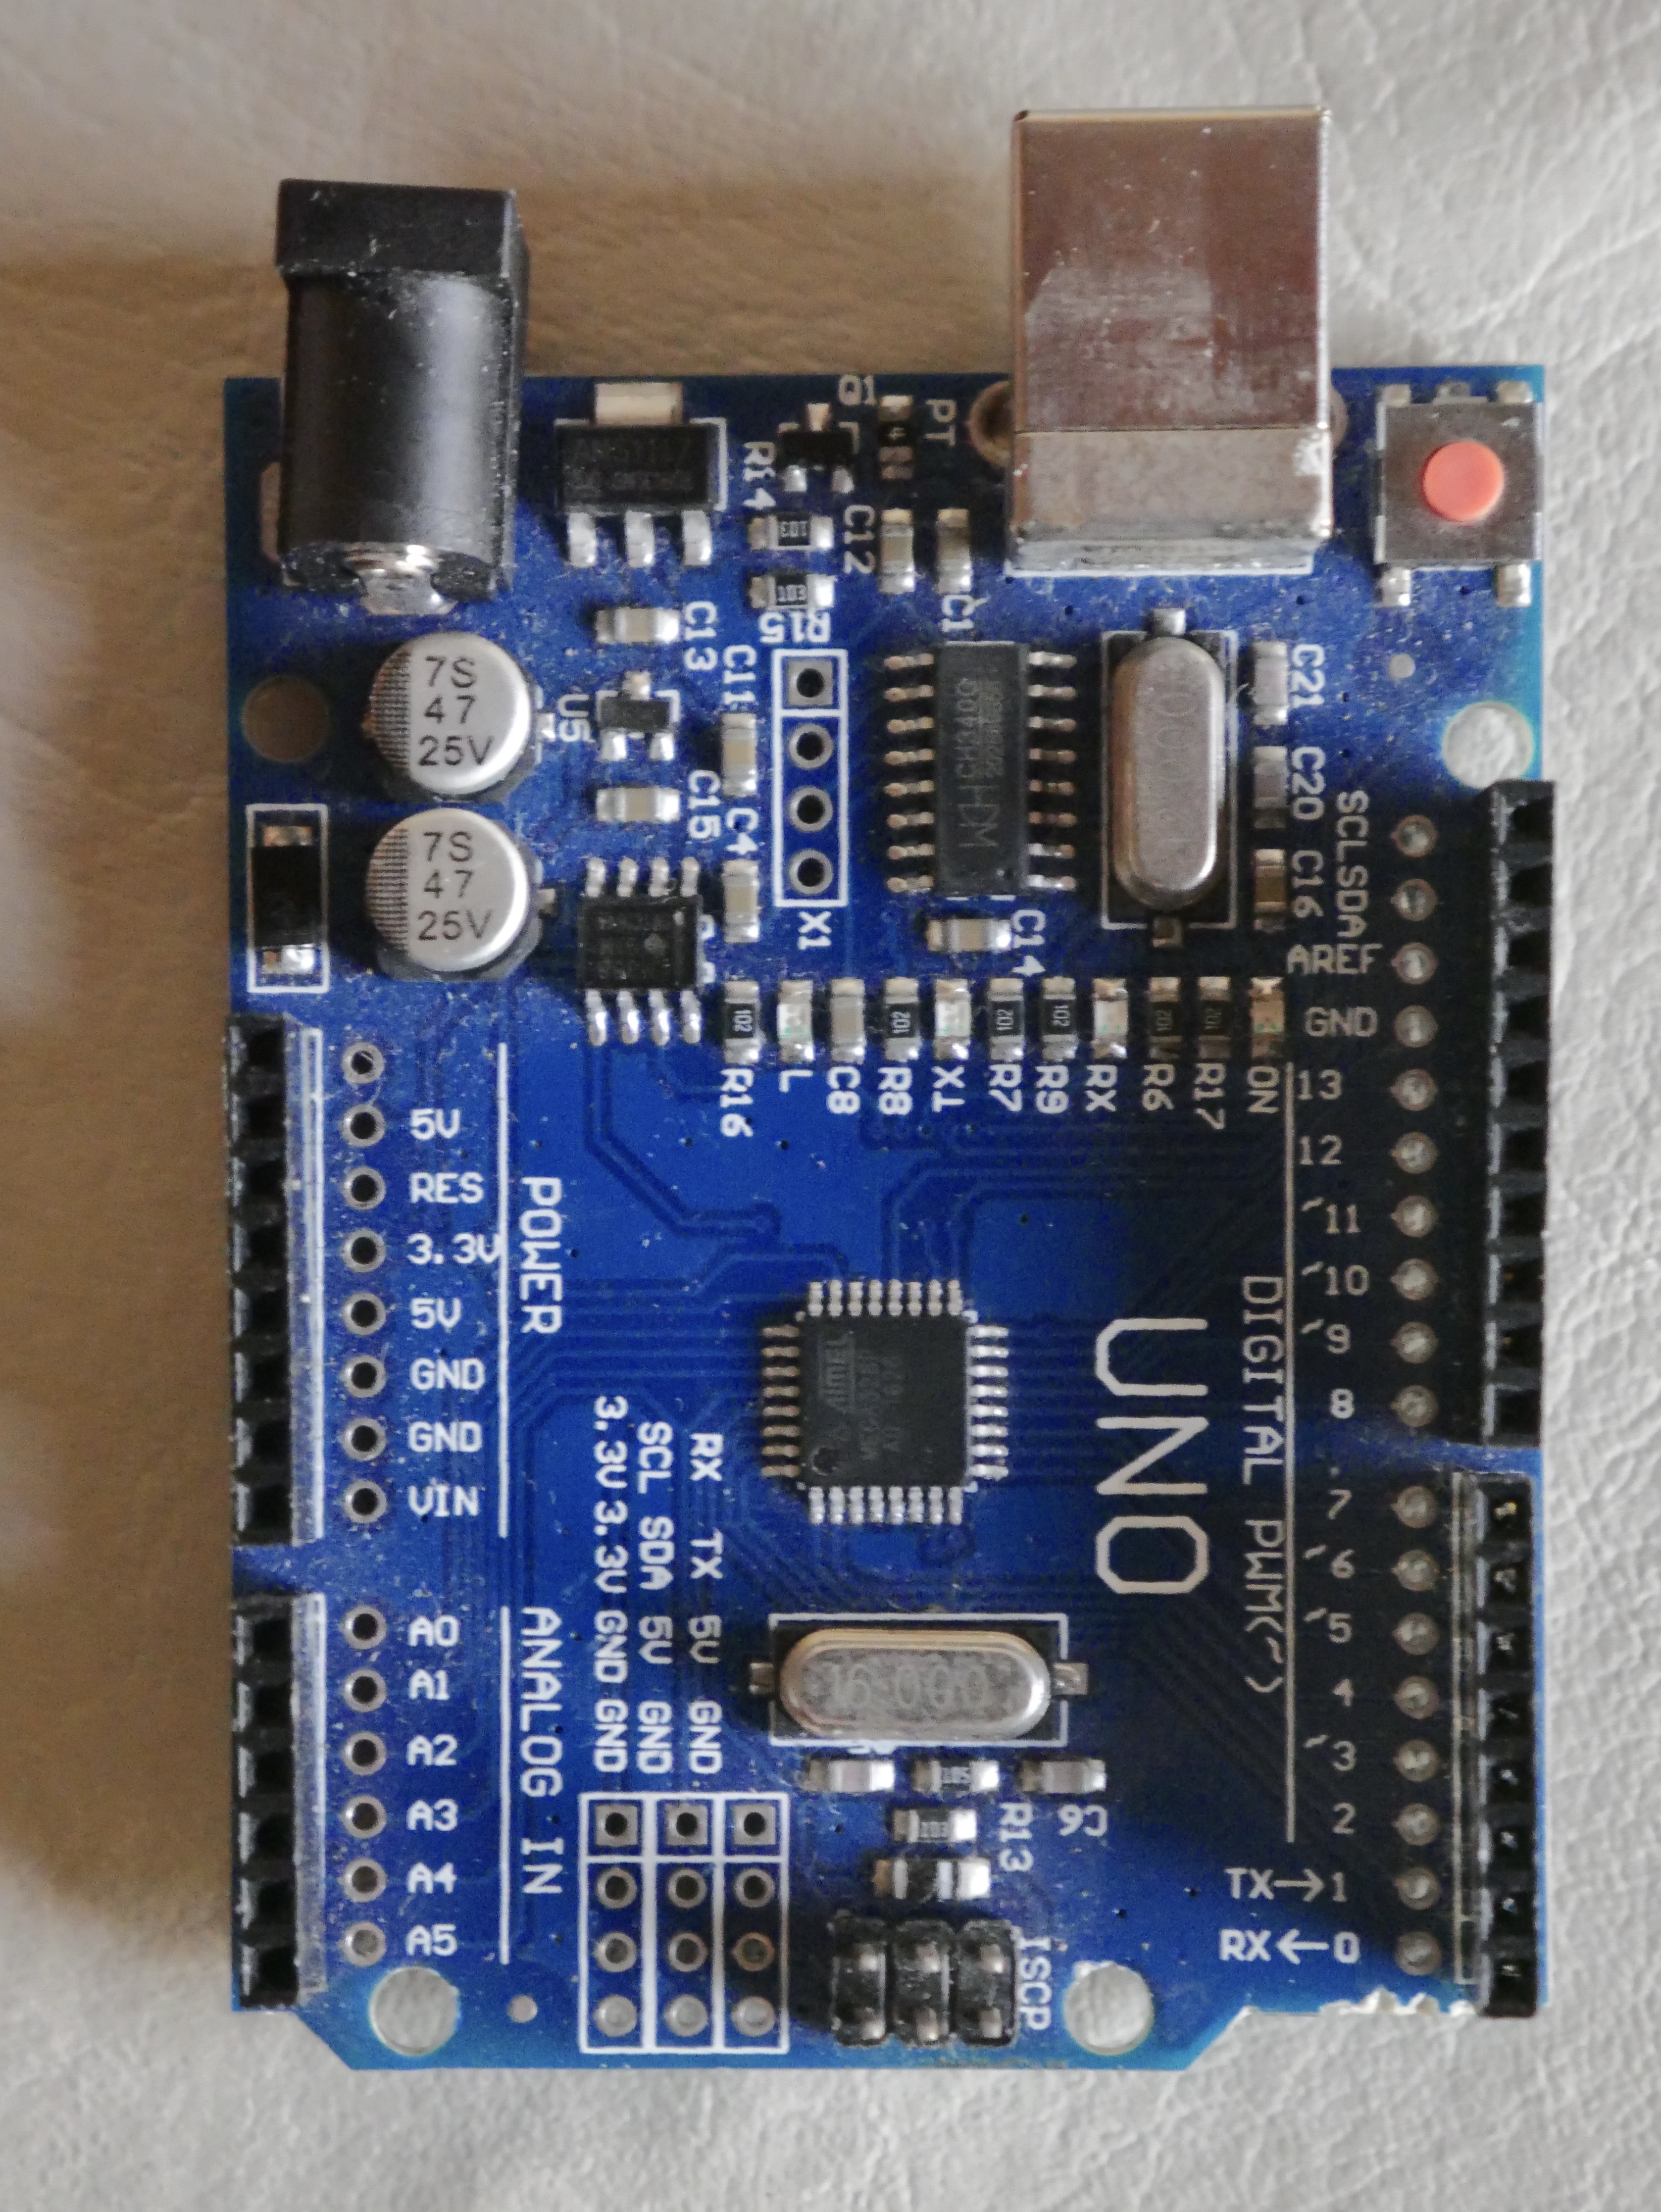
\includegraphics[width=.8\linewidth]{imagenes/IMG_0200.JPG}  
  \caption{Placa Arduino UNO utilizada}
  \label{fig:sub-first}
\end{minipage}
\begin{minipage}{.45\textwidth}
  \centering
  % include second image
  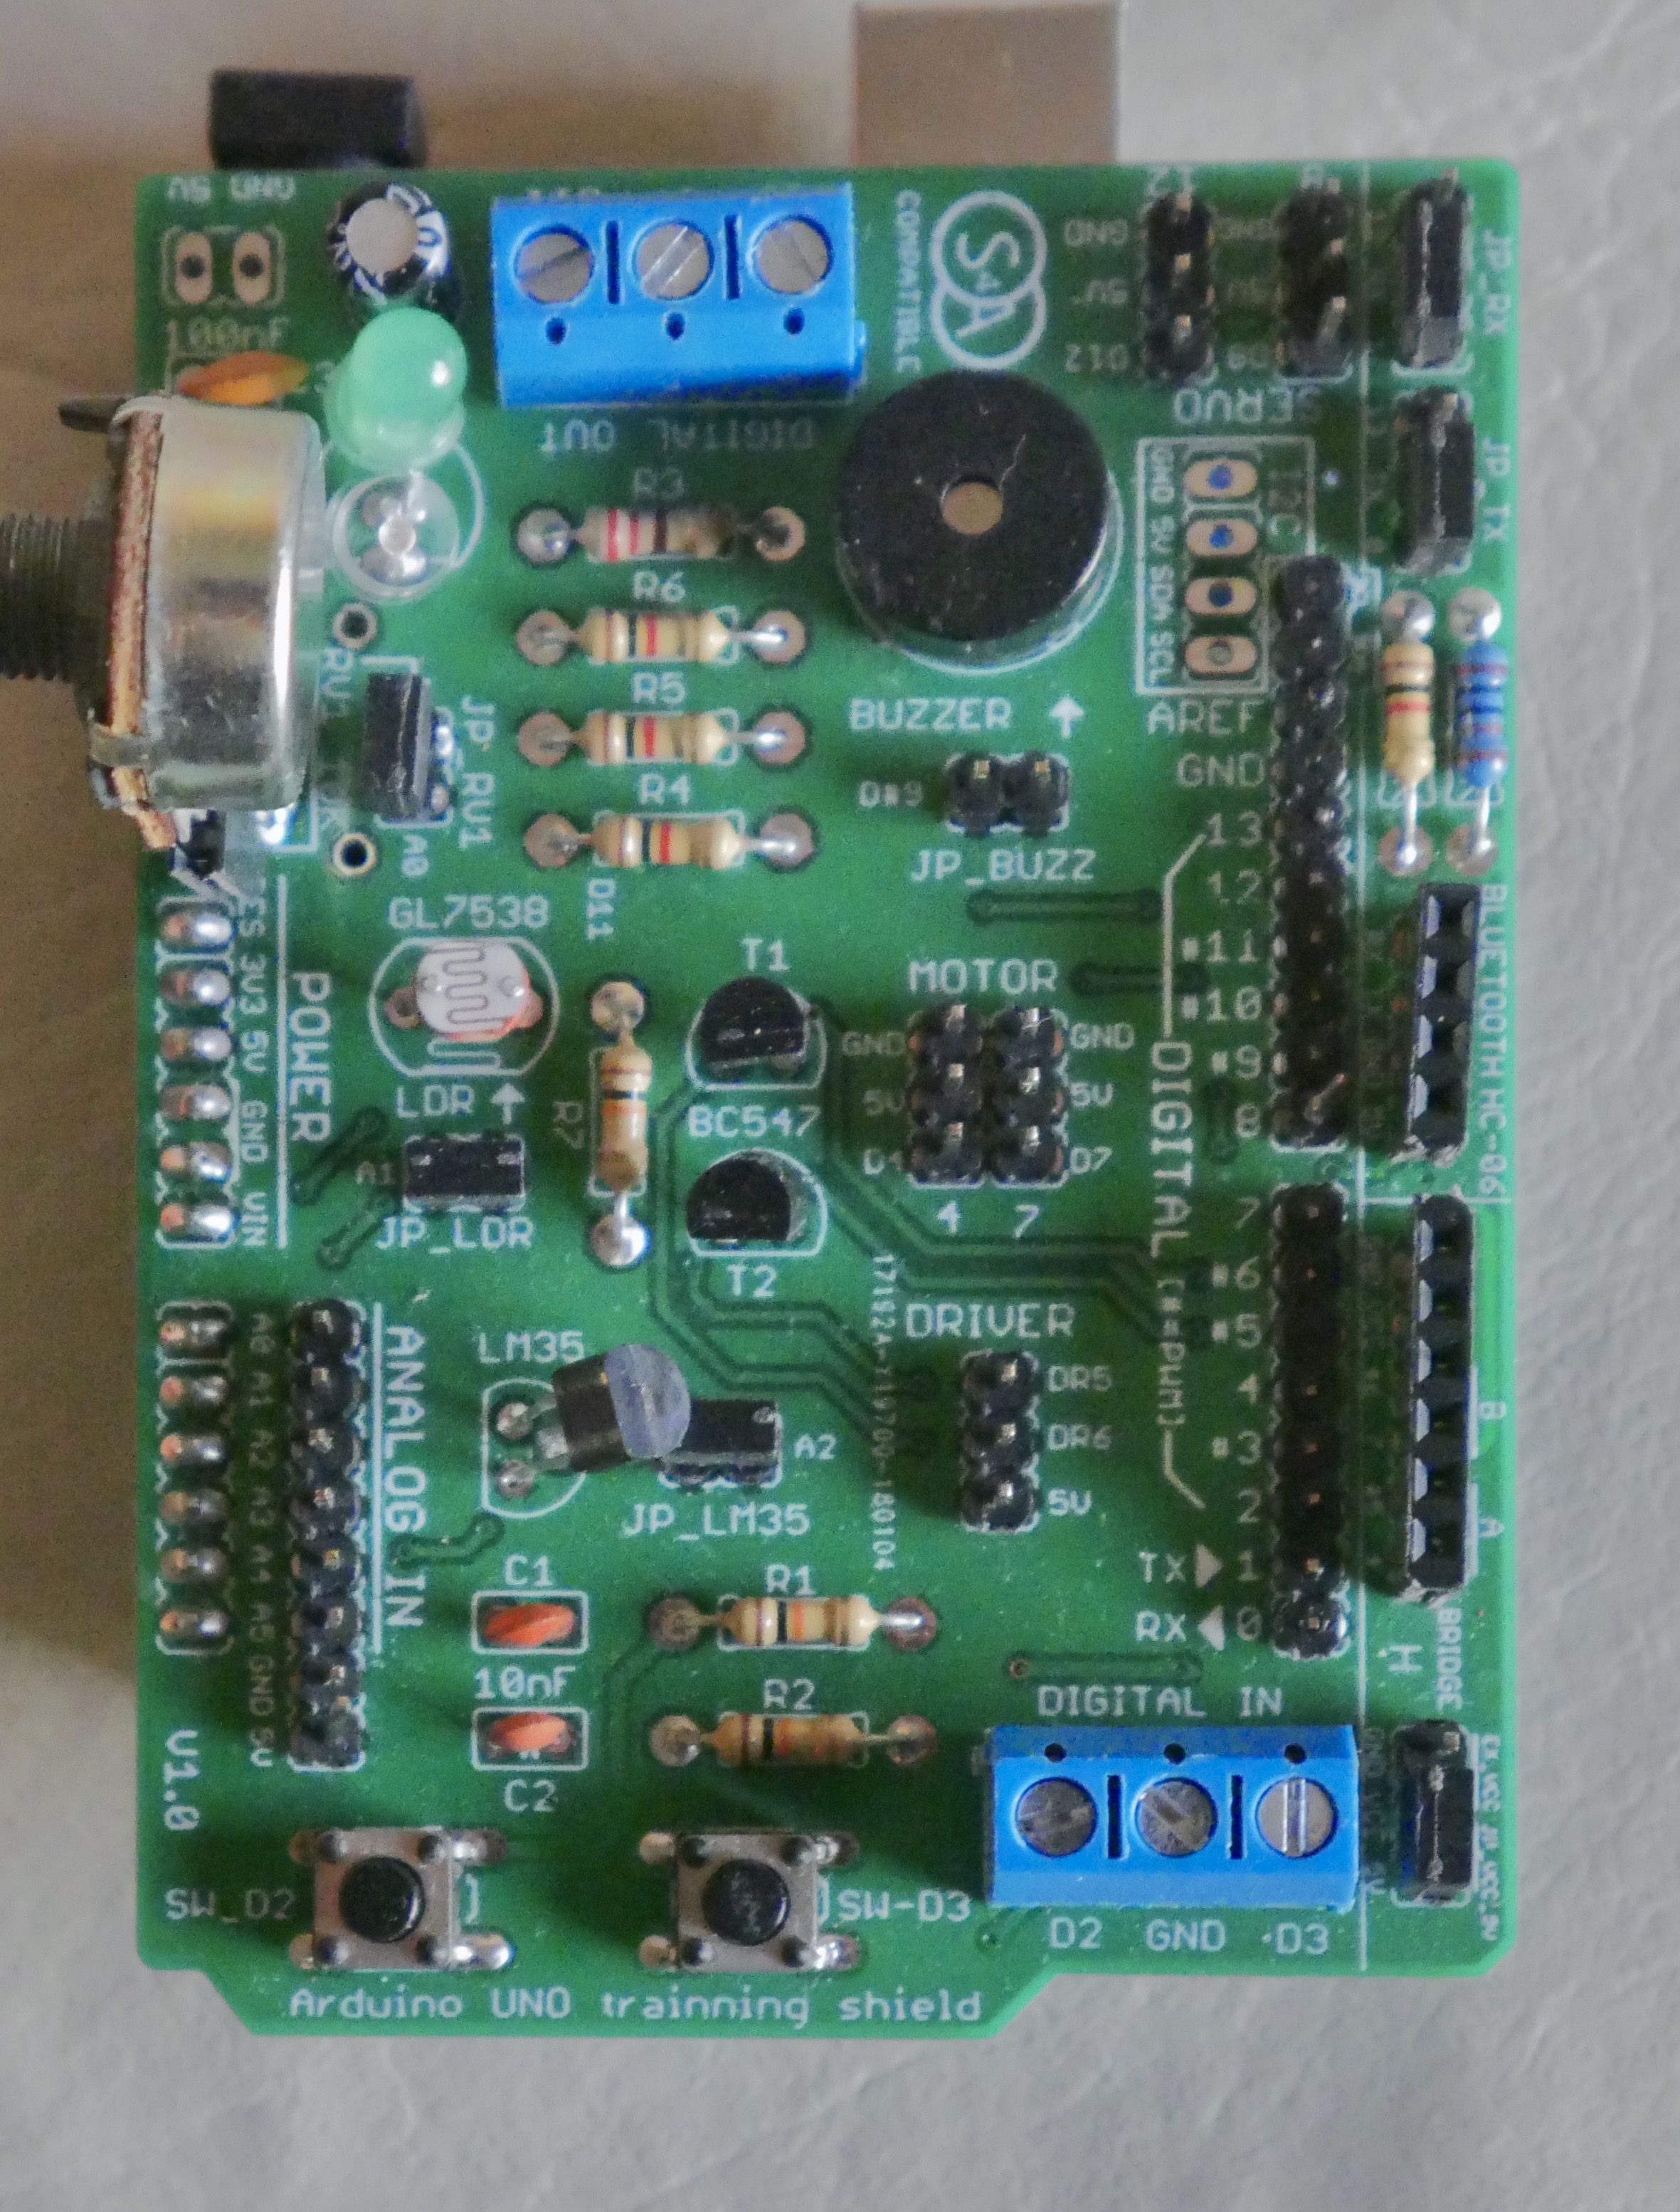
\includegraphics[width=.8\linewidth]{imagenes/IMG_0201.JPG}  
  \caption{Placa \textit{Shield I/O} utilizada para la conexión LED}
  \label{fig:sub-second}
\end{minipage}
\end{figure}

%%%%%%%%%%%%%%%%%%%%%%%%%%%%%%%%%%%%%%%%%%%%%%%%%%
\section{Diagrama  de conexión en bloques}
\begin{figure}[H]
    \centering
    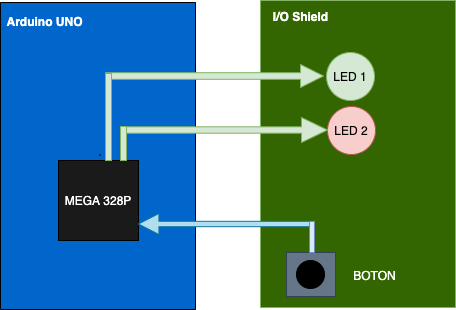
\includegraphics[width=9cm]{imagenes/TP4 Diagrama en bloques.png}
    \caption{Diagrama de conexión del hardware}
    \label{fig:conexion}
\end{figure}
%%%%%%%%%%%%%%%%%%%%%%%%%%%%%%%%%%%%%%%%%%%%%%%%%%%

\section{Circuito esquemático}

\begin{figure}[H]
    \centering
    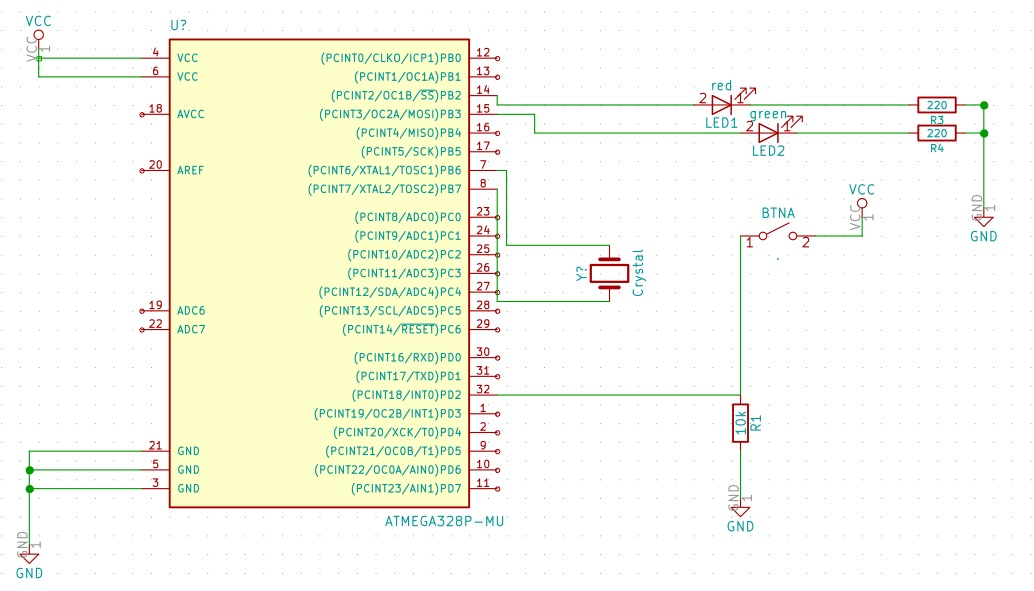
\includegraphics[width=0.7\linewidth]{imagenes/Circuito.jpg}
    \caption{Circuito esquemático}
    \label{fig:esquematico}
\end{figure}

\section{Listado de componentes y tabla de gastos}

\begin{table}[H]
    
    \centering
    \begin{tabular}{|c||c|}
    \hline
    \textbf{Componente}  & \textbf{Precio} \\ \hline \hline
    Arduino UNO & \$750  \\ \hline
    I/O Shield  & \$950  \\ \hline
    \end{tabular}
    \caption{Tabla de componentes}
    
\end{table}




\section{Software}


\begin{figure}[h]
    \centering
    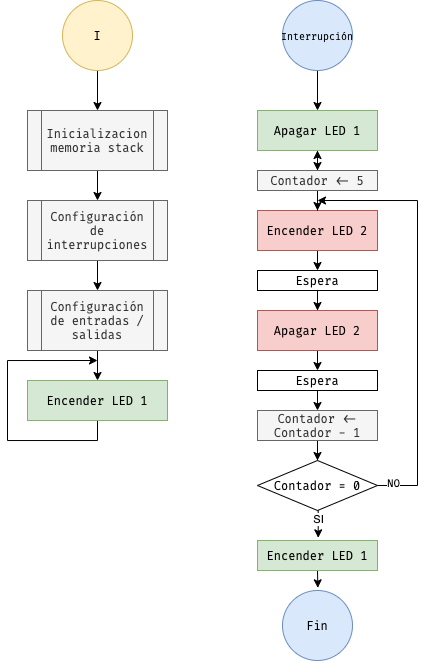
\includegraphics[width= 6 cm]{imagenes/TP4 Diagrama de flujo.png}
    \caption{Diagrama de flujo del programa e interrupción para controlar dos LED con botón pulsador}
    \label{fig:dflujo}
\end{figure}


El programa comienza con la configuración de los puertos B y D según la conexión del \textit{Shield} como salida y entrada respectivamente.
Luego, a diferencia de los trabajos anteriores, se realizó la configuración de las interrupciones. Esto consiste en cargar el registro \texttt{EICRA} con unos en los bits correspondientes a la interrupción \texttt{INT0}, de esta manera programando que la interrupción se realice con flanco ascendente.
Luego se cargo el registro \texttt{EIMSK} el cual se utiliza para activar las interrupciones, por lo que se activo la correspondiente a \texttt{INT0}. Habiendo así terminado la configuración correspondiente a interrupciones agregando la instrucción \texttt{SEI} en la subrutina llamada \textit{INIT\_INT0}, se procedió a la configuración de entrada y salida en la subrutina \textit{INIT\_HARDW}.
Luego se comienza con el \textit{loop} principal el cual solo consiste en encender el \textbf{LED 1}. 
La subrutina que corresponde a la interrupción, llamada \textit{parpadeo}, primero se llama a una subrutina llamada \textit{debounce} en la cual se realiza una pequeña espera y luego se hace una segunda lectura del pin de entrada, si la segunda lectura no coincide con la primera, se sale de la interrupción. Retomando con la rutina de interrupcion, luego, se apaga el \textbf{LED 1} y luego se hace parpadear el \textbf{LED 2} 5 veces con esperas de $500 \ms$ así logrando una frecuencia de parpadeo de $1 \Hz$.
Terminada la secuencia de parpadeo, se vuelve a encender el \textbf{LED 1} y así se termina la secuencia de interrupción, volviendo al \textit{loop} principal.


\section{Resultados}

Se logró realizar la animación y visualizar correctamente el comportamiento esperado. Aunque hubo dificultades el principio por haber omitido la instrucción \texttt{SEI}, esto provocó un comportamiento errático del circuito y en definitiva sin cumplir lo indicado. Luego de detectado este error, el circuito funcionó correctamente.
Por ultimo, se pregunta qué se modificaría si se cambian las resistencias de \textit{pull\-down} por \textit{pull\-up}, esto cambiaría el estado lógico normalmente leído por el circuito, por lo que en principio se tendría que cambiar el evento de lectura de flanco ascendente por descendente y luego ajustar la segunda lectura dentro la subrutina de \textit{debounce}. 
 

